\chapter{Empirical Study}\label{discover}\label{eval}


To characterize the location of logging usage in source code, I conducted an experimental study to address the following research questions: 

\begin{itemize} [leftmargin=.5in]
\item \textsc{RQ1: }\emph{``Is it possible to find patterns in where log statements do occur in source code?''} We aim to investigate whether there are clusters containing a large number of logged methods, meaning that there are common ways of locating log statements in source code.

\item \textsc{RQ2: }\emph{``What common structural characteristics do logged methods have?''} We aim to examine the logging usage schemas extracted by my tool to identify the common structural characteristics of logged methods. 
\end{itemize}


\section{Experiment}  \label{setup-characterization}
I applied my tool on the source code of five open-source software systems and extract the logging usage schemas on a per-system method-granularity basis analysis. The chosen systems are \code{Apache FTP Server}, \code{Hibernate ORM}, \code{Apache Camel}, \code{OpenMeetings}, and \code{QuickFIX/J}, all written in the Java programming languages and all utilized the same logging framework, \code{Apache Log4j}, which is ranked as the most commonly used logging package for Java\footnote{\url{https://en.wikipedia.org/wiki/Java_logging_framework}}.Table~\ref{au2_tab1} represents the details about these software systems. I believe that studying these Java projects could give us an insight about logging usage in real-world applications.

%, which are selected due to their popularity in their area of application\footnote{\url{}}\footnote{\url{}} and long history (at least ... years) in software development

% should be modified
\begin{center}
\begin{table} [H]
\begin{center}
    \begin{tabular}{ | l | l | c | c |}
    \hline
    \textbf{Software}  & \textbf{Description}   & \textbf{LOC} & \textbf{\# of methods}  \\ \hline
    {Apache FTP Server 1.0.0} & FTP server  & 98K  & 1865 \\ \hline
{Hibernate ORM 5.1} & Object relational-mapping framework & 508K &50712   \\ \hline
    {Apache Camel 2.17} &  Rule-based routing and mediation engine  &  120K &32293 \\ \hline
{OpenMeetings 2.0} & Web Conferencing & 38K &3506 \\ \hline
    {QuickFIX/J 1.6} & FIX engine  & 48K & 2958 \\ \hline
    \end{tabular}
    \caption{Details of the five open-source software systems that make use of the {Apache Log4j} logging framework.}
\label{au2_tab1}
\end{center}
\end{table}
\end{center}

My proof-of-concept implementation takes the source code of these Java projects as input, extracts ASTs of their LMs, applies the proposed algorithm to construct the AUASTs and classify them into clusters, and outputs the detailed view of structural generalization for each cluster, called logging usage schema. I decided to exclude log statements with the \emph{trace} and \emph{debug} verbosity level in my experiment, since they are usually used by developers only during the software development phase.


\section{Results}  \label{results-characterization}
The results of the experiment for each software system are presented in Table~\ref{tab_results_1} that describes the total number of detected \code{log4j} statements (debug- and trace-level log statements are excluded), the number of logged methods (LMs); the number of generated clusters; the number of singleton clusters that only contain one LM; the reduction percentage calculated by the Equation~\ref{reduction_eq}. In addition, Figure~\ref{fig:histograms} shows the histograms of the number of LMs per cluster for each system.
% to measure the feasibility of finding patterns in the usage of log statements.

\begin{figure} [H]
  \centering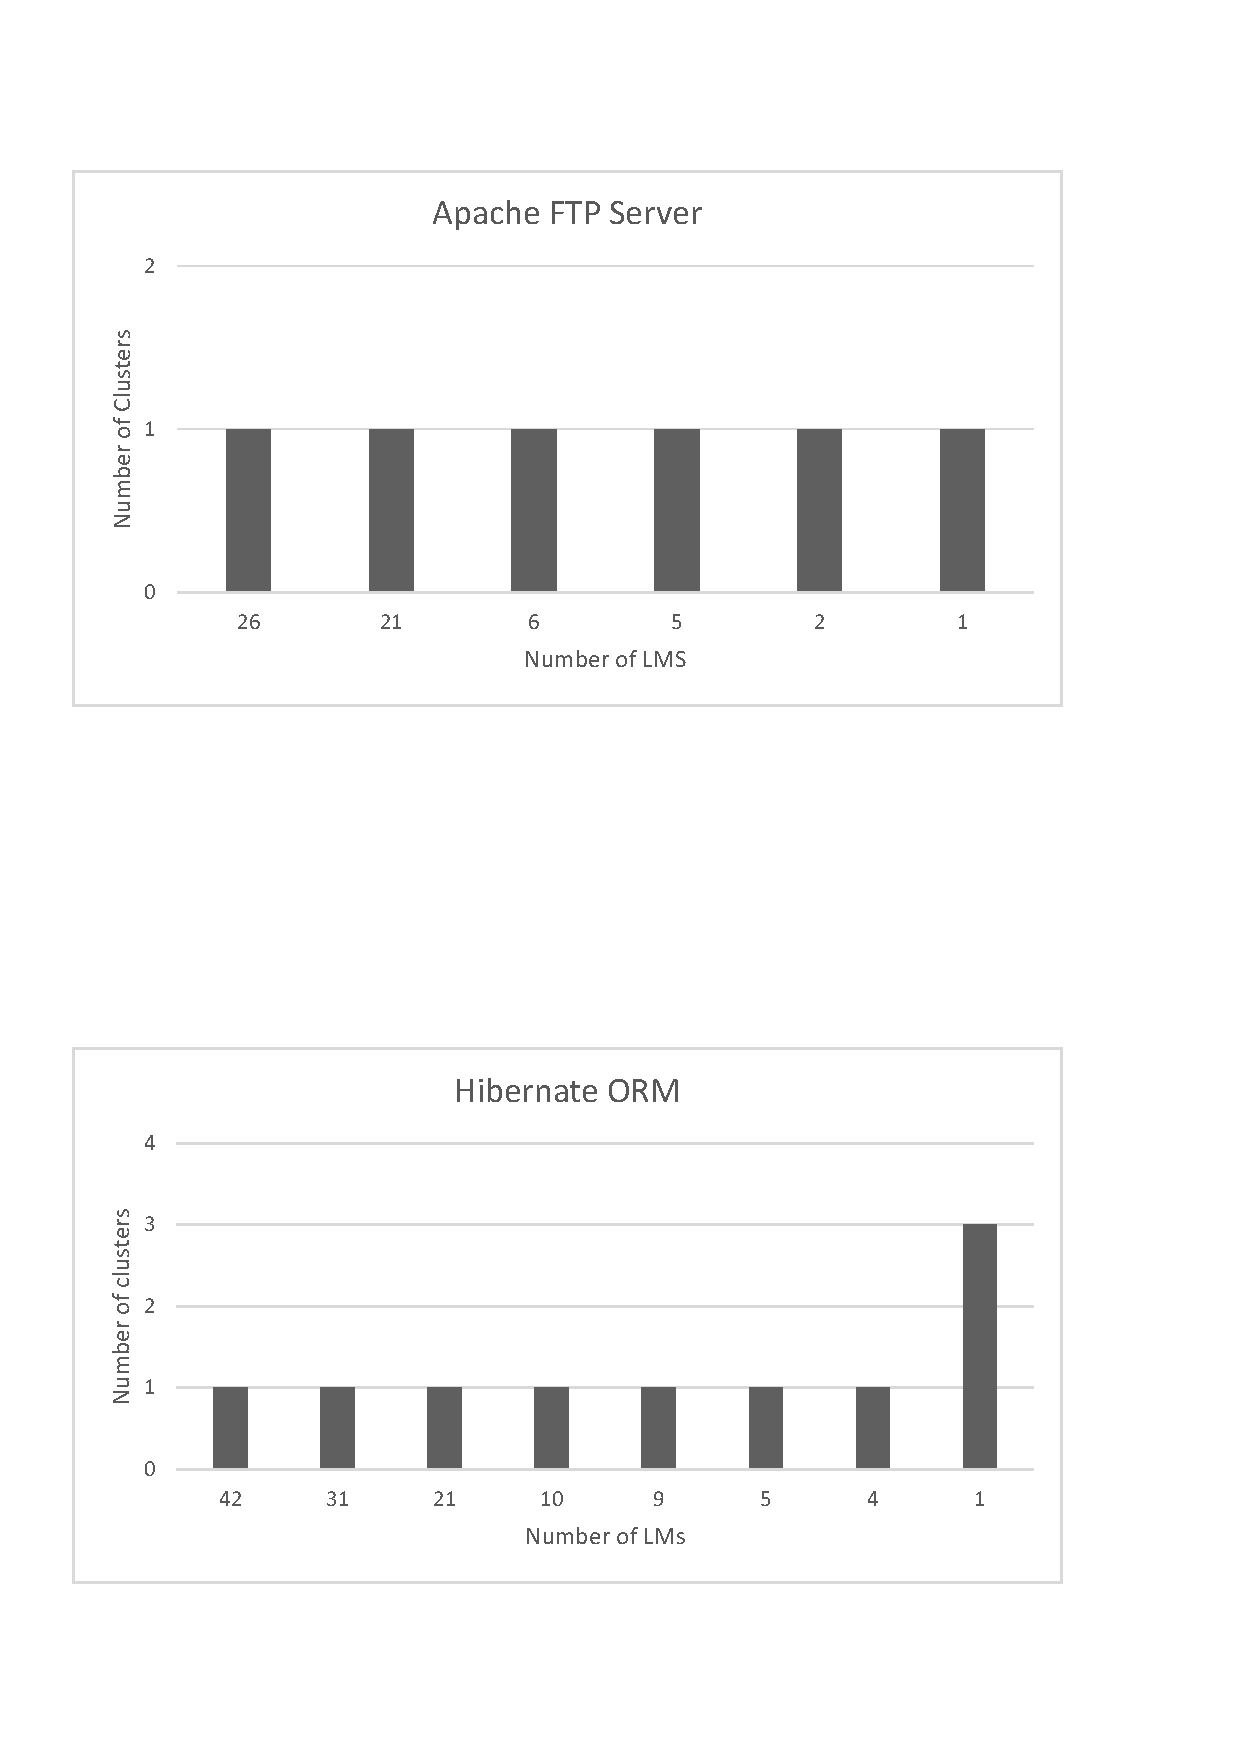
\includegraphics [width = 0.5\textwidth, height = 0.5\textheight]{Histograms/Histograms.pdf}
  \caption{Histograms of the number of LMS per cluster.}
  \label{fig:histograms}
\end{figure}

\begin{figure} [H]
  \centering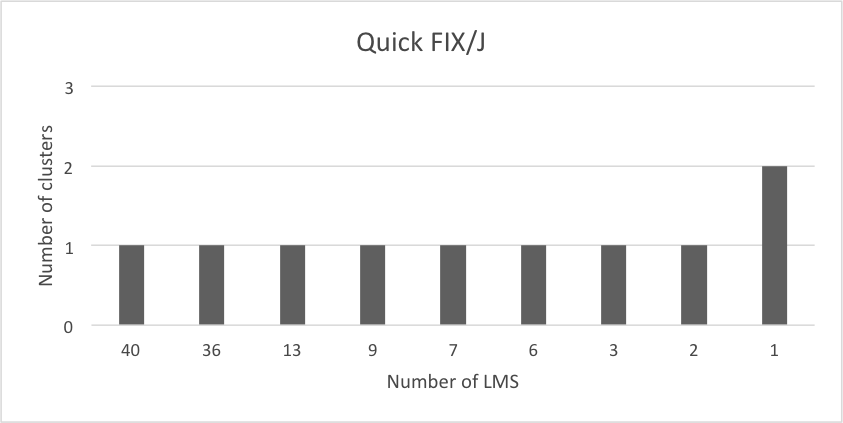
\includegraphics [width = 0.4\textwidth, height = 0.15\textheight]{Histograms/QUICK.png}
  \caption{Histograms of the number of LMS per cluster.}
  \label{fig:histograms}
\end{figure}

%{Drawing4/...}
%of clusters that contains a certain number of LMs in three software systems.
 %The reduction metric shows how much logged methods can be grouped together.%number of LMs that are generalized with another LMs in one cluster and its percentage of the total number of LMs;

\begin{equation}\label{reduction_eq}
%\mbox{reduction} = \frac{\mbox{\# of log statements} - \mbox{\# of clusters}}{\mbox{\# of log statements}}
\end{equation}

\begin{table}[h]
\vspace*{1em}
\let\A\relax
\newlength{\A} \settowidth{\A}{288}
\let\B\relax
\newlength{\B}
\settowidth{\B}{329}
\let\Cl\relax
\newlength{\Cl}
\settowidth{\Cl}{343}
\let\Ac\relax
\newlength{\Ac}
\settowidth{\Ac}{}
\let\Bc\relax
\newlength{\Bc}
\settowidth{\Bc}{}
\let\Abc\relax
\newlength{\Abc}
\settowidth{\Abc}{}
\let\Pwa\relax
\newlength{\Pwa}
\settowidth{\Pwa}{\%}
\centering\begin{tabular}{lccc}
  \toprule 
   & \multicolumn{1}{c}{Apache FTP Server}  & \multicolumn{1}{c}{Hibernate ORM} & \multicolumn{1}{c}{Apache Camel} \\
  \midrule
  Log4j statements          & \makebox[\Ac][c]{61}                                  & \makebox[\Bc][c]{125}                                  & \makebox[\Abc][c]{} \\\midrule
 LMs               & \makebox[\Ac][c]{39}                                  & \makebox[\Bc][c]{92}                                  & \makebox[\Abc][c]{330}\\

  Clusters  & \makebox[\Ac][c]{\makebox[\A][r]{6}}                 & \makebox[\Bc][c]{\makebox[\B][r]{10}}                 & \makebox[\Abc][c]{\makebox[\Cl][r]{}} \\


  Singleton clusters       & \makebox[\Ac][c]{\makebox[\A][r]{1}}                 & \makebox[\Bc][c]{\makebox[\B][r]{3}}                 & \makebox[\Abc][c]{\makebox[\Cl][r]{}} \\\midrule

  Reduction                       & \makebox[\Ac][c]{\makebox[\A][r]{90\%\hspace*{-\Pwa}}} & \makebox[\Bc][c]{\makebox[\B][r]{92\%\hspace*{-\Pwa}}} &\\
  \\
    \toprule 
  
& \multicolumn{1}{c}{OpenMeetings} & \multicolumn{1}{c}{QuickFIX/J}\\

\midrule

  Log4j statements            & \makebox[\Bc][c]{}                                  & \makebox[\Abc][c]{118} \\\midrule

 LMs               &  \makebox[\Abc][c]{624}& \makebox[\Abc][c]{96} \\

  Clusters  & \makebox[\Ac][c]{\makebox[\A][r]{}}                 & \makebox[\Bc][c]{\makebox[\B][r]{10}}                 & \makebox[\Abc][c]{\makebox[\Cl][r]{}} \\


  Singleton clusters       & \makebox[\Ac][c]{\makebox[\A][r]{}}                 & \makebox[\Bc][c]{\makebox[\B][r]{2}}                 & \makebox[\Abc][c]{\makebox[\Cl][r]{}} \\\midrule

  Reduction                       & \makebox[\Ac][c]{\makebox[\A][r]{\%\hspace*{-\Pwa}}} & \makebox[\Bc][c]{\makebox[\B][r]{91\%\hspace*{-\Pwa}}} &  
  
  
\end{tabular}
%\caption{Within-version experiment.}
\caption{Per-system evaluation results.}
%\caption{Experimental results for the the software systems}
\label{tab_results_1} \vspace*{1em}
\end{table}

\section{Evaluation}  \label{evaluation}


\begin{algorithm}
\caption{\func{Determine-Locations}($\id{antiUnifier}$,$\id{methods}$) finds the locations in source code that matches an anti-unifier.}
\label{alg-determine}
\begin{algorithmic}[1]
\DetermineLocations
    \State $\id{locations} \gets \func{()}$
    \For {$\id{method} \in \id{methods}$}
    \State $\id{result} \gets  \func{AntiUnify}(\id{antiUnfier},\id{method})$
		\If {$\func{Equals}(\id{result},\id{antiUnifier})$ }	
				 	\State{$\func{Append}(\id{method},\id{locations})$ }
		\EndIf 		
		\EndFor
 \Return $\id{locations} $  	
  \end{algorithmic}
\end{algorithm}

\begin{table}[h]
\vspace*{1em}
\let\A\relax
\newlength{\A} \settowidth{\A}{288}
\let\B\relax
\newlength{\B}
\settowidth{\B}{288}
\let\Cl\relax
\newlength{\Cl}
\settowidth{\Cl}{288}
\let\Ac\relax
\newlength{\Ac}
\settowidth{\Ac}{}
\let\Bc\relax
\newlength{\Bc}
\settowidth{\Bc}{}
\let\Abc\relax
\newlength{\Abc}
\settowidth{\Abc}{}
\let\Pwa\relax
\newlength{\Pwa}
\settowidth{\Pwa}{\%}
\centering\begin{tabular}{l ccc ccc ccc}
  \toprule 

& \multicolumn{3}{c}{Apache FTP Server} & \multicolumn{3}{c}{Hibernate ORM} & \multicolumn{3}{c}{Apache Camel} \\\cmidrule(lr){2-4}\cmidrule(lr){5-7}\cmidrule(lr){8-10} 

&TP&FP&FN&TP&FP&FN&TP&FP&FN\\
\midrule
Constrained                   &
\makebox[\A][r]{40}  & \makebox[\A][r]{27} & \makebox[\A][r]{21} & \makebox[\A][r]{100}  & \makebox[\A][r]{27} & \makebox[\A][r]{25} &\makebox[\A][r]{}  & \makebox[\A][r]{} & \makebox[\A][r]{}  \\
Unconstrained                   &
\makebox[\A][r]{60}  & \makebox[\A][r]{134} & \makebox[\A][r]{1} & \makebox[\A][r]{123}  & \makebox[\A][r]{184} & \makebox[\A][r]{2} &\makebox[\A][r]{}  & \makebox[\A][r]{} & \makebox[\A][r]{} 
\\
 \toprule 
 & \multicolumn{3}{c}{OpenMeetings}& \multicolumn{3}{c}{QuickFIX/J}\\\cmidrule(lr){2-4}\cmidrule(lr){5-7}

&TP&FP&FN&TP&FP&FN\\
\midrule
Constrained                   &
\makebox[\A][r]{}  & \makebox[\A][r]{} & \makebox[\A][r]{} &\makebox[\A][r]{91}  & \makebox[\A][r]{31} & \makebox[\A][r]{27} \\
Unconstrained                   &
\makebox[\A][r]{}  & \makebox[\A][r]{} & \makebox[\A][r]{} &\makebox[\A][r]{101}  & \makebox[\A][r]{75} & \makebox[\A][r]{17} \\


\end{tabular}
\caption{Per-system evaluation results.}
\label{tab_results_2} \vspace*{1em}
\end{table}

\begin{table}[h]
\vspace*{1em}
\let\A\relax
\newlength{\A} \settowidth{\A}{288}
\let\B\relax
\newlength{\B}
\settowidth{\B}{329}
\let\Cl\relax
\newlength{\Cl}
\settowidth{\Cl}{343}
\let\Ac\relax
\newlength{\Ac}
\settowidth{\Ac}{}
\let\Bc\relax
\newlength{\Bc}
\settowidth{\Bc}{}
\let\Abc\relax
\newlength{\Abc}
\settowidth{\Abc}{}
\let\Pwa\relax
\newlength{\Pwa}
\settowidth{\Pwa}{\%}
\centering\begin{tabular}{l cc cc cc}
  \toprule 

& \multicolumn{2}{c}{Apache FTP Server} & \multicolumn{2}{c}{Hibernate ORM} & \multicolumn{2}{c}{Apache Camel} \\\cmidrule(lr){2-3}\cmidrule(lr){4-5}\cmidrule(lr){6-7} 

 &Constrained & Unconstrained&Constrained &Unconstrained&Constrained & Unconstrained\\
\midrule

  Precision                       & \makebox[\Ac][c]{\makebox[\A][r]{59\%\hspace*{-\Pwa}}} & \makebox[\Bc][c]{\makebox[\B][r]{31\%\hspace*{-\Pwa}}} &  \makebox[\Ac][c]{\makebox[\A][r]{78\%\hspace*{-\Pwa}}} & \makebox[\Bc][c]{\makebox[\B][r]{40\%\hspace*{-\Pwa}}} &  \makebox[\Ac][c]{\makebox[\A][r]{\%\hspace*{-\Pwa}}}  &  \makebox[\Ac][c]{\makebox[\A][r]{\%\hspace*{-\Pwa}}}
  
  \\
  
 Recall                           & \makebox[\Ac][c]{\makebox[\A][r]{65\%\hspace*{-\Pwa}}} & \makebox[\Bc][c]{\makebox[\B][r]{98\%\hspace*{-\Pwa}}} &  \makebox[\Ac][c]{\makebox[\A][r]{80\%\hspace*{-\Pwa}}} & \makebox[\Bc][c]{\makebox[\B][r]{98\%\hspace*{-\Pwa}}} &  \makebox[\Ac][c]{\makebox[\A][r]{\%\hspace*{-\Pwa}}}  &  \makebox[\Ac][c]{\makebox[\A][r]{\%\hspace*{-\Pwa}}}
 
 \\
 \toprule
 & \multicolumn{2}{c}{OpenMeetings}& \multicolumn{2}{c}{QuickFIX/J}\\\cmidrule(lr){2-3}\cmidrule(lr){4-5}

&Constrained &Unconstrained&Constrained & Unconstrained\\
\midrule

  Precision                       & \makebox[\Bc][c]{\makebox[\B][r]{\%\hspace*{-\Pwa}}}& \makebox[\Ac][c]{\makebox[\A][r]{\%\hspace*{-\Pwa}}} & \makebox[\Bc][c]{\makebox[\B][r]{75\%\hspace*{-\Pwa}}}& \makebox[\Bc][c]{\makebox[\B][r]{53\%\hspace*{-\Pwa}}}
  
  \\
  
 Recall                           & \makebox[\Bc][c]{\makebox[\B][r]{\%\hspace*{-\Pwa}}}& \makebox[\Ac][c]{\makebox[\A][r]{\%\hspace*{-\Pwa}}} & \makebox[\Bc][c]{\makebox[\B][r]{77\%\hspace*{-\Pwa}}}& \makebox[\Bc][c]{\makebox[\B][r]{85\%\hspace*{-\Pwa}}}


\end{tabular}
%\caption{Within-version experiment.}
\caption{Per-system evaluation results.}
\label{tab_results_3} \vspace*{1em}
\end{table}



\section{Analysis}  \label{analysis}
The first research question is : \emph{"Is it possible to find patterns in where log statements do occur in source code?"}. As it is shown in Table~\ref{tab_results_1}, the reduction value for all software systems are above 90\%, indicating that most LMs are grouped together in a single cluster. Furthermore, histograms depicted in Figure~\ref{fig:histograms}  indicates that ...


To address the second research question, I manually examined the logging usage schemas for each system to extract the commonalities amongst logged methods of each cluster. 

%\section{Lessons Learned}  \label{Lessons-Learned}
\

\section{Summary}
I conducted an experimental study to characterize the location of log statements through the application of my tool on the source code of five full software systems that make use of the \code{Log4j} logging framework. My tool inputs the source code of these systems, extracts ASTs of LMs, applies the proposed anti-unification and clustering algorithms, and outputs the logging usage schema for each cluster. I also conducted an experimental study to evaluate the accuracy of the tool support in constructing the anti-unifiers that describe the location of log statements in source code. The results taken form the characterization experiment shows that there are common ways of locating log statements in source code. I manually examined the structural generalization schemas to figure out common structural characteristics of logged methods in each cluster. I found out that most log statements are embedded inside ....
